\documentclass[a4paper]{article}
\usepackage[english]{babel}
\usepackage[utf8]{inputenc}
\usepackage{textcomp}
\usepackage{amsmath}
\usepackage{gensymb}
\usepackage{physics}
\usepackage{graphicx}
\usepackage[colorinlistoftodos]{todonotes}
\usepackage{xcolor}
\usepackage{array}
\usepackage{tabularx}
\usepackage{tikz}
\usepackage{pgfplots}
\usepackage{framed}
\usepackage{xfrac}
\usepackage[most]{tcolorbox}
\usepackage{fix-cm}
\usepackage{cancel}
\usepackage[margin=0.5in]{geometry}
\usetikzlibrary{quotes,angles}
\usetikzlibrary{decorations.pathreplacing}
\usetikzlibrary{calc}
\usepgfplotslibrary{fillbetween}

\let\phi\varphi
\let\bf\textbf
\colorlet{shadecolor}{orange!15}
\pgfplotsset{compat=1.18}
\newcommand\der[2]{\frac{d #1}{d #2}}
\newcommand\Deltat{\Delta t}
\newcommand\rads{\text{ rad\;s}^{-1}}
\newcommand\radss{\text{ rad\;s}^{-2}}
\newcommand\rad{\text{ rad}}
\newcommand\s{\text{ s}}
\newcommand\m{\text{ m}}
\newcommand\J{\text{ J}}
\newcommand\Nm{\text{ Nm}}
\newcommand\ms{\text{ ms}^{-1}}
\newcommand\mss{\text{ ms}^{-2}}
\newcommand\kg{\text{ kg}}
\newcommand\kgms{\text{ kg\;ms}^{-1}}
\newcommand\kgmm{\text{ kg\;m}^{2}}
\newcommand{\AxisRotator}[1][rotate=0]{%
    \tikz [x=0.25cm,y=0.60cm,line width=.2ex,-stealth,#1] \draw (0,0) arc (-150:150:1 and 1);%
}
\def\centerarc[#1](#2)(#3:#4:#5){\draw[#1] ($(#2)+({#5*cos(#3)},{#5*sin(#3)})$) arc (#3:#4:#5)}
% Syntax: \centerarc[draw options] (center) (initial angle:final angle:radius);

\title{Angular Momentum}
\author{OpenStax University Physics Vol. 1}
\date{}

\begin{document}
\setcounter{section}{11}
\maketitle
\subsection{Rolling Motion}
Rolling motion is the common combinatipno of rotational and translational motion seen every day, such as wheels moving on a car along a highway or wheels on a plane landing on a runway.\vspace{2mm}\\
\bf{Rolling Motion Without Slipping}\vspace{2mm}\\
Rolling motion without slipping has been observed since the invention of the wheel. For example, consider the interaction of a car's tires and the surface of the road. If the driver floors the accelerator such that the tires spin without moving the car, there must be kinetic friction between the wheels and the surface of the road. If the driver depresses the accelerator slowly causing the car to move forward, then the tires roll without slipping. In fact the bottom of the wheel is at rest with respect to the ground, indicating there must be static friction between the tires and the road surface.\vspace{1mm}\\
To analyze rolling without slipping, we first derive the linear variables of velocity and acceleration of the center of mass of the wheel in terms of the angular variables that describe the wheel's motion, shown below.

\begin{center}
    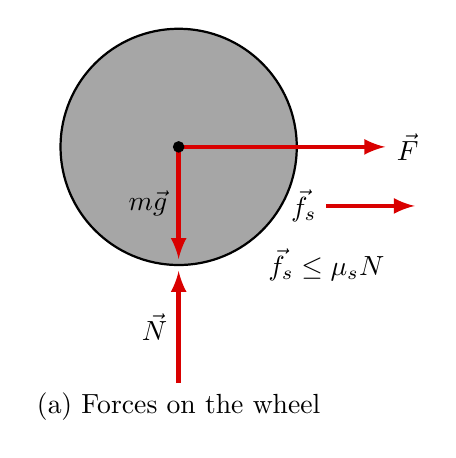
\begin{tikzpicture}[scale=1.5]
        \filldraw[black!35] (0,0) circle (1);
        \draw[black,thick] (0,0) circle (1);

        \draw[->,ultra thick,-latex,black!15!red] (0,0)--node[left,text=black]{$m\vec{g}$}(0,-0.95);
        \draw[->,ultra thick,-latex,black!15!red] (0,-2)--node[left,text=black]{$\vec{N}$}(0,-1.05);
        \draw[->,ultra thick,-latex,black!15!red] (0,0)--(1.75,0) node[right,text=black]{$\vec{F}$};
        \draw[->,ultra thick,-latex,black!15!red] (1.25,-0.5)--(2,-0.5);
        \node[left] at (1.25,-0.5){$\vec{f}_s$};
        \node at (1.25,-1){$\vec{f}_s \leq \mu_sN$};

        \filldraw[black] (0,0) circle  (1.25pt);
        \node at (0,-2.2){(a) Forces on the wheel};
    \end{tikzpicture}
    \hspace{5mm}
    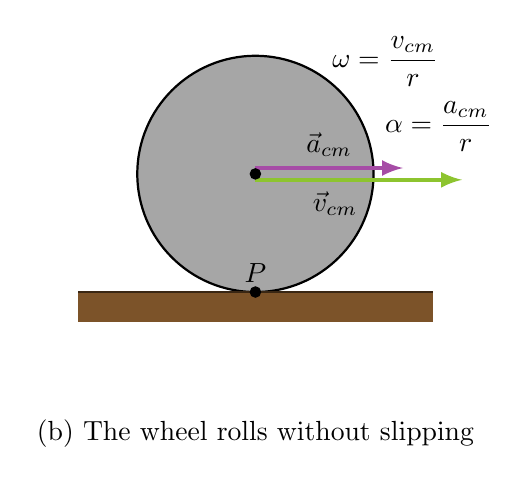
\begin{tikzpicture}[scale=1.5]
        \filldraw[black!35] (0,0) circle (1);
        \draw[black,thick] (0,0) circle (1);

        \draw[->,ultra thick,-latex,black!15!yellow!60!green] (0,-0.05)--node[below,text=black,xshift=-3mm]{$\vec{v}_{cm}$} (1.75,-0.05);
        \draw[->,ultra thick,-latex,white!30!violet] (0,0.05)--node[above,text=black]{$\vec{a}_{cm}$} (1.25,0.05);
        \filldraw[black!35!brown] (-1.5,-1) rectangle (1.5,-1.25);
        \draw[line width=0.5pt,draw=black!70!brown] (-1.5,-1)--(1.5,-1);

        \filldraw[black] (0,-1) circle (1.25pt) node[above]{$P$};
        \filldraw[black] (0,0) circle (1.25pt);
        \centerarc[<-,very thick,latex-,black](0,0)(150:225:1.25);

        \node at (1.1,0.95){$\displaystyle \omega = \frac{v_{cm}}{r}$};
        \node at (1.55,0.4){$\displaystyle \alpha = \frac{a_{cm}}{r}$};
        \node at (0,-2.2){(b) The wheel rolls without slipping};
    \end{tikzpicture}
    \hspace{5mm}
    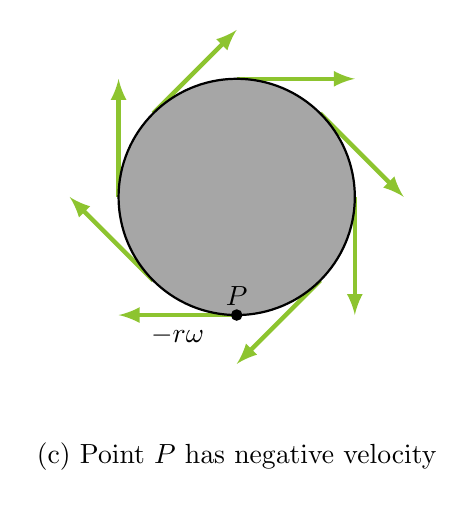
\begin{tikzpicture}[scale=1.5]
        \draw (0,1) coordinate (a);
        \draw (1,0) coordinate (b);
        \draw (0,-1) coordinate (c);
        \draw (-1,0) coordinate (d);
        \draw ({cos(45)},{sin(45)}) coordinate (e);
        \draw ({cos(45)},{-sin(45)}) coordinate (f);
        \draw ({-cos(45)},{-sin(45)}) coordinate (g);
        \draw ({-cos(45)},{sin(45)}) coordinate (h);

        \draw[->,ultra thick,-latex,black!15!yellow!60!green] (a)--([turn]-90:1);
        \draw[->,ultra thick,-latex,black!15!yellow!60!green] (b)--([turn]-90:1);
        \draw[->,ultra thick,-latex,black!15!yellow!60!green] (c)-- node[below,text=black]{$-r\omega$} ([turn]-90:1);
        \draw[->,ultra thick,-latex,black!15!yellow!60!green] (d)--([turn]-90:1);
        \draw[->,ultra thick,-latex,black!15!yellow!60!green] (e)--([turn]-90:1);
        \draw[->,ultra thick,-latex,black!15!yellow!60!green] (f)--([turn]-90:1);
        \draw[->,ultra thick,-latex,black!15!yellow!60!green] (g)--([turn]-90:1);
        \draw[->,ultra thick,-latex,black!15!yellow!60!green] (h)--([turn]-90:1);

        \filldraw[black!35] (0,0) circle (1);
        \draw[black,thick] (0,0) circle (1);
        \filldraw[black] (0,-1) circle (1.25pt) node[above]{$P$};

        \node at (0,-2.2){(c) Point $P$ has negative velocity};
    \end{tikzpicture}
\end{center}
In (a), we see the force vectors involved in preventing the wheel from slipping. In (b), the point $P$ that touches the surface is at rest relative to the surface. Relative to the center of mass, point $P$ has velocity $-r\omega\hat{i}$, where $r$ is the radius of the wheel and $\omega$ is the wheel's angular velocity about its axis. Since the wheel is rolling, the velocity of $P$ with respect to the surface is its velocity with respect to the center of mass plus the velocity of the center of mass with respect to the surface:
\begin{align*}
    \vec{v}_P = -r\omega\hat{i} + v_{cm}\hat{i}
\end{align*}
Since the velocity of $P$ relative to the surface is zero, $v_P = 0$, this says that:
\begin{equation}
    v_{cm} = r\omega
\end{equation}
The velocity of the wheel's center of mass is its radius times the angular velocity about its axis. Differentiating the left side of the equation gives an expression for the linear acceleration of the center of mass, on the right side, $r$ is constant and since $\alpha = \der{\omega}{t}$:
\begin{equation}
    a_{cm} = r\alpha
\end{equation}
Further, the distance the wheel travels can be found in terms of angular variables. As the wheel rolls from point $A$ to point $B$, its outer surface maps onto the ground by exactly the distance traveled $d_{cm}$. The length of the outer surface that maps onto the ground is the arc length $r\theta$. Equating the two distances gives:
\begin{equation}
    d_{cm} =  r\theta
\end{equation}
\begin{center}
    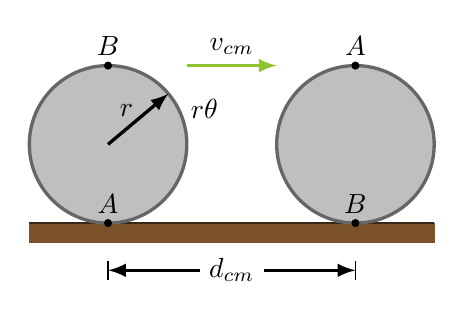
\begin{tikzpicture}[scale=1]
        %%% Ground %%%
        \filldraw[black!35!brown] (-1,-1) rectangle (4.1415,-1.25);
        \draw[line width=0.5pt,draw=black!70!brown] (-1,-1)--(4.1415,-1);

        %%% Circle 1 %%%
        \filldraw[black!25] (0,0) circle (1);
        \draw[black!60,very thick] (0,0) circle (1);
        \filldraw[black] (0,1) circle (1.25pt) node[above]{$B$};
        \filldraw[black] (0,-1) circle (1.25pt) node[above]{$A$};
        \draw[->,very thick,-latex] (0,0)--node[above,xshift=-1.5mm,yshift=-1mm]{$r$} ({cos(40)},{sin(40)});
        \node at ({1.3*cos(20)},{1.3*sin(20)}){$r\theta$};
        \centerarc[->,black!5!green!50!blue,very thick,latex-](0,0)(270:450:1);

        %%% Circle 2 %%%
        \filldraw[black!25] (3.1415,0) circle (1);
        \draw[black!60,very thick] (3.1415,0) circle (1);
        \filldraw[black] (3.1415,1) circle (1.25pt) node[above]{$A$};
        \filldraw[black] (3.1415,-1) circle (1.25pt) node[above]{$B$};
        \centerarc[-,black!5!green!50!blue,very thick](3.1415,0)(90:270:1);

        %%% d_{cm} %%%
        \draw[<->,very thick,latex-latex] (0,-1.6)--node[fill=white]{$d_{cm}$}(3.1415,-1.6);
        \draw[line width=0.5pt] (0,-1.48)--(0,-1.72);
        \draw[line width=0.5pt] (3.1415,-1.48)--(3.1415,-1.72);

        %%% v_{cm} %%%
        \draw[->,very thick,-latex,draw=black!15!yellow!60!green] (1,1)--node[above]{$v_{cm}$}(2.1415,1);
    \end{tikzpicture}
\end{center}

\begin{shaded}
    \underline{\bf{Example 11.1:} Rolling Down an Inclined Plane}
    \vspace{2mm}\\
    A solid cylinder rolls down an inclined plane without slipping, starting from rest. It has mass $m$ and radius $r$.
    \begin{enumerate}
        \item[(a)] What is its acceleration?
        \vspace{1mm}\\
        There is barely enough friction to keep the cylinder rolling without slipping. Since there is no slipping, the magnitude of the friction force is $f_s \leq \mu_sN$. Writing down Newton's laws in the $x$ and $y$ direction we have:
        \begin{align*}
            \sum F_x = ma_x\ \text{ and }\ \sum F_y = ma_y
        \end{align*}
        \begin{center}
            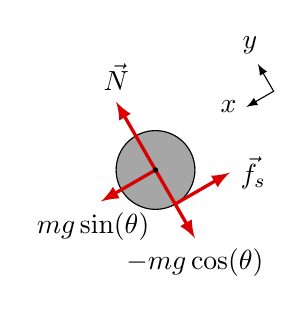
\begin{tikzpicture}
                \filldraw[black!35] (0,0) circle (0.5);
                \draw[black] (0,0) circle (0.5);

                \draw[->,very thick,draw=black!15!red,-latex] (0,0)--({-cos(60)},{sin(60)}) node[above]{$\vec{N}$};
                \draw[->,very thick,draw=black!15!red,-latex] (0,0)--({-0.8*cos(30)},{-0.8*sin(30)}) node[below,xshift=-1mm]{$mg\sin(\theta)$};
                \draw[->,very thick,draw=black!15!red,-latex] (0,0)--({cos(60)},{-sin(60)}) node[below]{$-mg\cos(\theta)$};
                \draw[->,very thick,draw=black!15!red,-latex] ({0.5*cos(60)},{-0.5*sin(60)})--({0.5*cos(60) + 0.8*cos(30)},{-0.5*sin(60) + 0.8*sin(30)}) node[right]{$\vec{f}_s$};

                \filldraw (0,0) circle (0.75pt);

                \draw[->,latex-latex] ({1.5 - 0.4*cos(30)},{1 - 0.4*sin(30)})--(1.5,1)--({1.5 - 0.4*cos(60)},{1 + 0.4*sin(60)}) node[above,xshift=-1mm]{$y$};
                \node[left] at ({1.5 - 0.4*cos(30)},{1 - 0.4*sin(30)}){$x$};
            \end{tikzpicture}
        \end{center}
        Substituting in from the free-body diagram:
        \begin{align*}
            mg\sin(\theta) - f_s &= m(a_{cm})\\
            N - mg\cos(\theta) &= 0
        \end{align*}
        The linear acceleration can then be solved for the linear acceleration of the center of mass using the equation
        \begin{align*}
            a_{cm} = g\sin(\theta) - \frac{f_s}{m}.
        \end{align*}
        However, it is useful to express the linear acceleration in terms of the moment of inertia, for this, use Newton's second law for rotation
        \begin{align*}
            \sum\tau_{cm} = I_{cm}\alpha
        \end{align*}
        The torques are calculated about the axis through the center of mass of the cylinder. The only nonzero torque is provided by the friction force:
        \begin{align*}
            f_sr = I_{cm}\alpha
        \end{align*}
        Finally, the linear acceleration is related to the angular acceleration by $a_{cm,x} = r\alpha$. These equations can be used to solve for $a_{cm}, \alpha,$ and $f_s$ in terms of the moment of inertia. $a_{cm}$ is rewritten in terms of the vertical component of gravity and the friction force, and the following substitutions are made:
        \begin{align*}
            f_s = \frac{I_{cm}\alpha}{r} = \frac{I_{cm}a_cm}{r^2}
        \end{align*}
        Substituting this in for $f_s$ in the equation above, gives:
        \begin{align*}
            a_{cm} &= g\sin(\theta) - \frac{I_{cm}a_{cm}}{mr^2}\\
            &= \frac{mg\sin(\theta)}{m + (\sfrac{I_{cm}}{r^2})}
        \end{align*}
        Therefore:
        \begin{align*}
            \alpha = \frac{a_{cm}}{r} = \frac{2}{3r}g\sin(\theta)
        \end{align*}
        \item[(b)] What condition must the coefficient of static friction $\mu_s$ satisfy so the cylinder does not slip?\vspace{2mm}\\
        Because slipping does not occur, $f_s \leq \mu_sN$. Solving for the friction force $f_s$,
        \begin{align*}
            f_s = I_{cm}\frac{\alpha}{r} = I_{cm}\frac{a_{cm}}{r^2} = \frac{I_{cm}}{r^2}\bigg(\frac{mg\sin(\theta)}{m + (\sfrac{I_{cm}}{r^2})}\bigg) = \frac{mgI_{cm}\sin(\theta)}{mr^2 + I_{cm}}
        \end{align*}
        Substituting in the condition for no slipping and noting that $N = mg\cos(\theta)$, gives
        \begin{align*}
            \frac{mgI_{cm}\sin(\theta)}{mr^2 + I_{cm}} \leq \mu_smg\cos(\theta)\ \text{ or }\ \mu_s \geq \frac{\tan(\theta)}{1 + (\sfrac{mr^2}{I_{cm}})}
        \end{align*}
        For the solid cylinder this becomes:
        \begin{align*}
            \mu_s \geq \frac{\tan(\theta)}{1 + (\sfrac{2mr^2}{mr^2})} = \frac{1}{3}\tan(\theta)
        \end{align*}
    \end{enumerate}
\end{shaded}
\newpage\noindent
It is worthwile to repeat the equation derived in the example for the acceleration of an object rolling without slipping:
\begin{equation}
    a_{cm} = \frac{mg\sin(\theta)}{1 + (\sfrac{I_{cm}}{r^2})}
\end{equation}
This equation is very useful for solving problems involving rolling without slipping. Note that the acceleration is less thana that of an object sliding down a frictionless plane with no rotation. The acceleration will also be different for two rotating objects with different rotational inertias.
\vspace{2mm}\\
\bf{Rolling Motion With Slipping}
\vspace{2mm}\\
In the case of rolling motion with slipping, we must use the coefficient of kinetic friction, which gives rise to the kinetic friction force since static friction is not present. In the case of slipping, $v_{cm} - r\omega \neq 0$, because the point $P$ on the wheel is not at rest on the surface, and $v_P \neq 0$. In this scenerio, $\omega \neq \frac{v_{cm}}{r}$ and $\alpha \neq \frac{a_{cm}}{r}$
\begin{center}
    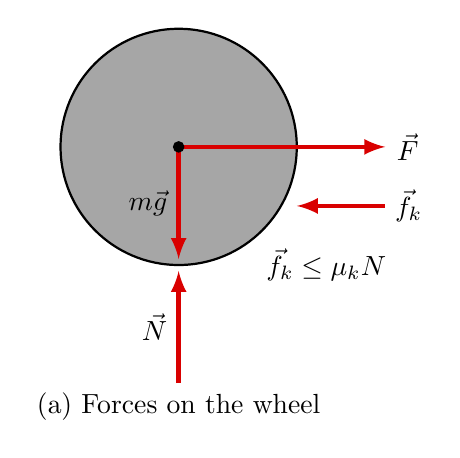
\begin{tikzpicture}[scale=1.5]
        \filldraw[black!35] (0,0) circle (1);
        \draw[black,thick] (0,0) circle (1);

        \draw[->,ultra thick,-latex,black!15!red] (0,0)--node[left,text=black]{$m\vec{g}$}(0,-0.95);
        \draw[->,ultra thick,-latex,black!15!red] (0,-2)--node[left,text=black]{$\vec{N}$}(0,-1.05);
        \draw[->,ultra thick,-latex,black!15!red] (0,0)--(1.75,0) node[right,text=black]{$\vec{F}$};
        \draw[->,ultra thick,latex-,black!15!red] (1,-0.5)--(1.75,-0.5);
        \node[right] at (1.75,-0.5){$\vec{f}_k$};
        \node at (1.25,-1){$\vec{f}_k \leq \mu_kN$};

        \filldraw[black] (0,0) circle  (1.25pt);
        \node at (0,-2.2){(a) Forces on the wheel};
    \end{tikzpicture}
    \hspace{5mm}
    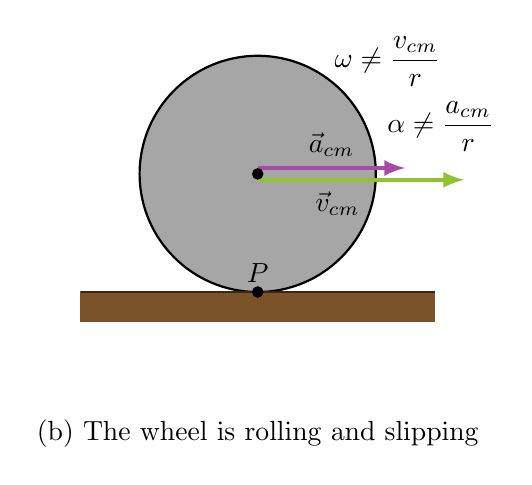
\begin{tikzpicture}[scale=1.5]
        \filldraw[black!35] (0,0) circle (1);
        \draw[black,thick] (0,0) circle (1);

        \draw[->,ultra thick,-latex,black!15!yellow!60!green] (0,-0.05)--node[below,text=black,xshift=-3mm]{$\vec{v}_{cm}$} (1.75,-0.05);
        \draw[->,ultra thick,-latex,white!30!violet] (0,0.05)--node[above,text=black]{$\vec{a}_{cm}$} (1.25,0.05);
        \filldraw[black!35!brown] (-1.5,-1) rectangle (1.5,-1.25);
        \draw[line width=0.5pt,draw=black!70!brown] (-1.5,-1)--(1.5,-1);

        \filldraw[black] (0,-1) circle (1.25pt) node[above]{$P$};
        \filldraw[black] (0,0) circle (1.25pt);
        \centerarc[<-,very thick,latex-,black](0,0)(150:225:1.25);

        \node at (1.1,0.95){$\displaystyle \omega \neq \frac{v_{cm}}{r}$};
        \node at (1.55,0.4){$\displaystyle \alpha \neq \frac{a_{cm}}{r}$};
        \node at (0,-2.2){(b) The wheel is rolling and slipping};
    \end{tikzpicture}
\end{center}

\begin{shaded}
    \underline{\bf{Example 11.2:} Rolling Down an Inclined Plane With Slipping}
    \vspace{2mm}\\
    A solid cylinder rolls down an inclined plane from rest and undergoes slipping. It has a mass $m$ and a radius $r$.\vspace{1mm}\\
    Draw a skech and free-body diagram showing the forces involved. The free-body diagram is similar to the no-slipping case except for the friction force, which is kinetic rather than static. Use Newton's second law to solve for the acceleration in the $x$ direction, and use Newton's second law of rotation to solve for the angular acceleration
    \begin{center}
        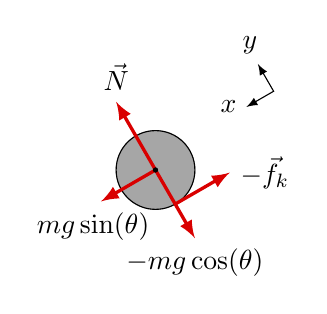
\begin{tikzpicture}
            \filldraw[black!35] (0,0) circle (0.5);
            \draw[black] (0,0) circle (0.5);

            \draw[->,very thick,draw=black!15!red,-latex] (0,0)--({-cos(60)},{sin(60)}) node[above]{$\vec{N}$};
            \draw[->,very thick,draw=black!15!red,-latex] (0,0)--({-0.8*cos(30)},{-0.8*sin(30)}) node[below,xshift=-1mm]{$mg\sin(\theta)$};
            \draw[->,very thick,draw=black!15!red,-latex] (0,0)--({cos(60)},{-sin(60)}) node[below]{$-mg\cos(\theta)$};
            \draw[->,very thick,draw=black!15!red,-latex] ({0.5*cos(60)},{-0.5*sin(60)})--({0.5*cos(60) + 0.8*cos(30)},{-0.5*sin(60) + 0.8*sin(30)}) node[right]{$-\vec{f}_k$};

            \filldraw (0,0) circle (0.75pt);

            \draw[->,latex-latex] ({1.5 - 0.4*cos(30)},{1 - 0.4*sin(30)})--(1.5,1)--({1.5 - 0.4*cos(60)},{1 + 0.4*sin(60)}) node[above,xshift=-1mm]{$y$};
            \node[left] at ({1.5 - 0.4*cos(30)},{1 - 0.4*sin(30)}){$x$};
        \end{tikzpicture}
    \end{center}
    \begin{enumerate}
        \item[(a)] What is its linear acceleration?\\
        The sum of the forces in the $y$ direction is zero, so the friction force is $f_k = \mu_kN = \mu_k$\\
        Newton's second law in the $x$ direction becomes:
        \begin{align*}
            \sum F_x &= ma_x\\
            mg\sin(\theta) - \mu_kmg&\cos(\theta) = ma_{cm,x}
        \end{align*}
        Which rearranges to 
        \begin{align*}
            a_{cm,x} = g\big(sin(\theta) - \mu_k\cos(\theta)\big)
        \end{align*}
        \item[(b)] What is its angular acceleration about an axis through the center of mass?\\
        The friction force provides the only torque about the axis through the center of mass, so Newton's second law of rotation becomes:
        \begin{align*}
            \sum\tau_{cm} &= I_{cm}\alpha\\
            f_kr &= I_{cm}\alpha = \frac{1}{2}mr^2\alpha
        \end{align*}
        Solving or $\alpha$ gives:
        \begin{align*}
            \alpha = \frac{2f_k}{mr} = \frac{2\mu_kg\cos(\theta)}{r}
        \end{align*}
    \end{enumerate}
\end{shaded}
\newpage

\noindent\bf{Conservation of Mechanical Energy in Rolling Motion}
\vspace{2mm}\\
Any rolling object carries rotational kinetic energy, as well as translational kinetic energy and potential energy if the system requires. Including the gravitational potential energy, the total mechanical energy of a rolling object is:
\begin{align*}
    E_T = \frac{1}{2}mv^2_{cm} + \frac{1}{2}I_{cm}\omega^2 + mgh
\end{align*}
In the absence of any nonconservative forces that would take energy out of the system in the form of heat, the total energy of a rolling object without slipping is conserved and is constant throughout the motion. In a rolling object that is slipping, energy is not conserved, the production of heat is the result of kinetic friction and a rolling object encountering air resistance.\vspace{1mm}\\
You may ask why a rolling object that is not slipping conserves energy, since the static friction force is nonconservative. The answer relates to the figure where point $P$ is shown in contact with the surface and at rest relative to the surface. Therefore the infinitesimal displacement $d\vec{r}$ with respect to the surface is zero and the incremental work done by the static friction is zero.
\begin{shaded}
    \underline{\bf{Example 11.3} Curiosity Rover}
    \vspace{2mm}\\
    The Curiosity rover was deployed on Mars on August 6, 2012. The wheels of the rover have a radius of 25 cm. Suppose astronauts arrive on Mars in the year 2050 and find the now inoperative Curiosity on the side of a basin. While they are dismantling the rover, an astronaut accidentially loses grip of one of the wheels, which rolls without slipping down into the bottom of the basin 25 meters below. If the wheel has a mass of 5 kg, what is its velocity at the bottom of the basin?\vspace{1mm}\\
    To solve the problem, use conservation of mechanical energy. At the top of the hill, the wheel is at rest and has only potential energy, at the bottom is has rotational and translational kinetic energy which must be equal to the initial potential energy. Since the wheel rolls without slipping, $v_{cm} = r\omega$.
    \vspace{1mm}\\
    The energy at the top is equal to the energy at the bottom:
    \begin{align*}
        mgh = \frac{1}{2}mv_{cm}^2 + \frac{1}{2}I_{cm}\omega^2
    \end{align*}
    The known quantities are $I_{cm} = mr^2$, $r = 0.25$ m, and $f = 25.0$ m. Rewriting the energy conservation equation, to solve for $v_{cm}$, eliminating $\omega$ using $\omega = \frac{v_{cm}}{r^2}$ gives:
    \begin{align*}
        mgh &= \frac{1}{2}mv_{cm}^2 + \frac{1}{2}mr^2\frac{v_{cm}^2}{r^2}\\
        gh &= \frac{1}{2}v_{cm}^2 + \frac{1}{2}v_{cm}^2\\
        v_{cm} &= \sqrt{gh}
    \end{align*}
    On Mars, the acceleration of gravity is 3.71$mss$, which gives the magnitude of velocity at the bottom of the basin as:
    \begin{align*}
        v_{cm} = \sqrt{\big(3.71\mss\big)(25.0\m)} = 9.63\ms
    \end{align*}
\end{shaded}

\end{document}